\chapter{Model implementation}
\label{chapter 5}
This chapter describes how the Navier Stokes numerical solver is actually constructed. We will talk about the spatial discretisation and implementation in Python. For clarity we will illustrate the numerical steps based on the Projection method with a lagged pressure approximation (Alg 2). Some of the ideas in the spatial discretisation part are based on Roberts' report on Navier stokes numerical solvers, including the use of ghost nodes on staggered grid. The code is also available upon request.

\section{Finite difference scheme}
This section is concerned with the implementation of second order Finite difference schemes. In the previous chapters we have only considered time discretisations whereas in this section we will describe how the spatial discretisation is done in order to fully illustrate our numerical solver.\\

The idea of spatial discretisation is to divide the domain which contains infinitely many ``points" into finite set of discrete cells or volumes. Then popular numerical techniques such as Finite difference and Finite volume methods can be used to approximate the continuous operators (e.g. Differentiation and Integration) based on the discrete cells.\\

There are many ways in which spatial discretisation can be done. Finite difference is one of the most simplest methods. Because our concern is mainly on the accuracy of different projection methods, hence Finite different method is advantageous over other methods because of its easy implementation yet providing robust computation efficiency. There are of course disadvantages associated with using Finite difference schemes, including the inability to handle complex geometries. Other more sophisticated methods including Finite elements and Finite volume methods can handle complex geometries but requires more complicated implementations. For instance, Finite element methods requires the use of Weak formulation of Navier Stokes equations. We leave these drawbacks as potential improvements in future researches.\\

The idea of finite differencing comes from using known function values to approximate derivatives and integrals. For instance if our domain is an unit square, then we can divide it into $n \times n$ many cells each with width $\Delta x = \Delta y = \dfrac{1}{n}$. Then the function values and their derivatives can be calculated on these points. The width or step size ($\Delta x$) are important in the outcome of the numerical approximation. Small step size or finer grids usually gives better approximations and smaller (spatial) error.

\subsection{Approximation to derivatives}
The use of finite differencing to approximate derivatives are commonly used in numerical studies and simulations. The formula is derived from a simple Taylor expansion of the function $f(x,y,t)$. Suppose we want to find the first $x$ derivative of $f$ at location $(i,\,j)$ which corresponds to ($x= i \Delta x,\, y= i\Delta y$) using a second order centred differencing scheme. We use the nearby function values at $i+1$ and $i-1$ to do so. The index $i,j$ ranges from $0$ to $n,m$ respectively. Please not be confused with time iterations ``n". Now Let's Taylor expand $f_{i+1,j}$ and $f_{i-1,j}$ at $f_{i,j}$
\begin{equation*}
f_{i+1,j} = f_{i,j} + f'_{i,j}\,(\Delta x)+\dfrac{f''_{i,j}\,(\Delta x)^2}{2} + \mathcal{O}(\Delta x^3)
\end{equation*}
\begin{equation*}
f_{i-1,j} = f_{i,j} - f'_{i,j}\,(\Delta x)+\dfrac{f''_{i,j}\,(\Delta x)^2}{2} + \mathcal{O}(\Delta x^3)
\end{equation*}
Using $f_{i+1,j} - f_{i-1,j}$ to eliminate the second derivatives:
\begin{equation*}
\dfrac{\partial f}{\partial x} = f'_{i,j} = \dfrac{f_{i+1,j} - f_{i-1,j}}{2\Delta x} + \mathcal{O}(\Delta x^2)
\end{equation*}
This is called ``centered finite differencing" or 2 - point stencil (since 2 points are involved in calculations) and it is clearly of second order accurate. The derivative in $y$  and $t$ uses the same approach.\\

The second order and higher derivatives can be derived using the same Taylor expansion argument. For instance
\begin{equation*}
\dfrac{\partial^2 f}{\partial x^2} = f''_{i,j} = \dfrac{f_{i+1,j} - f_{i,j} + f_{i-1,j}}{\Delta x^2} + \mathcal{O}(\Delta x^2)
\end{equation*}

It is quite straightforward to generalise this Finite differencing schemes to higher order accuracy. However more points are involved as we go up the order in Taylor series. This introduces many practical problems including larger stencils which would make the implementation harder. Then the idea of ``Compact Finite difference" comes into play where the derivatives at a set of points are solved by a linear system. This guarantees high order of accuracy without working with too many points. A 3 point stencil is often used when approximating the first derivative to 4th order accuracy. However it is not our focus point in this project and hence we leave this to future researches.

\subsection{Staggered grid}
To this end, we have been working with grids where the function values (and its derivatives) for both velocity and pressure variables are stored at the same locations. Usually they are evaluated at the vertices (or centre) of the square cells. This is called ``non-staggered" mesh grid or ``collocated" grid. This the most ``intuitive way" to think about the spatial discretisation, however this also introduces many problems including odd even grid decoupling because the pressure gradient and divergence terms are non-elliptic at grid scale \cite{armfield2000fractional}. This is because the variables are not stored in optimal locations. First introduced by Harlow, Francis H, Welch and J Eddie, staggered grid solves this issue quite nicely \cite{harlow1965numerical}.\\

Now with a staggered grid geometry, the variables are separated to different locations to avoid the odd-even grid decoupling. The scalar variable Pressure values are stored in the cell centres whereas the velocity variables are located at the cell faces. A picture of the staggered grid extracted from Robert's report is shown below:

\begin{figure}[H]
	\centering
	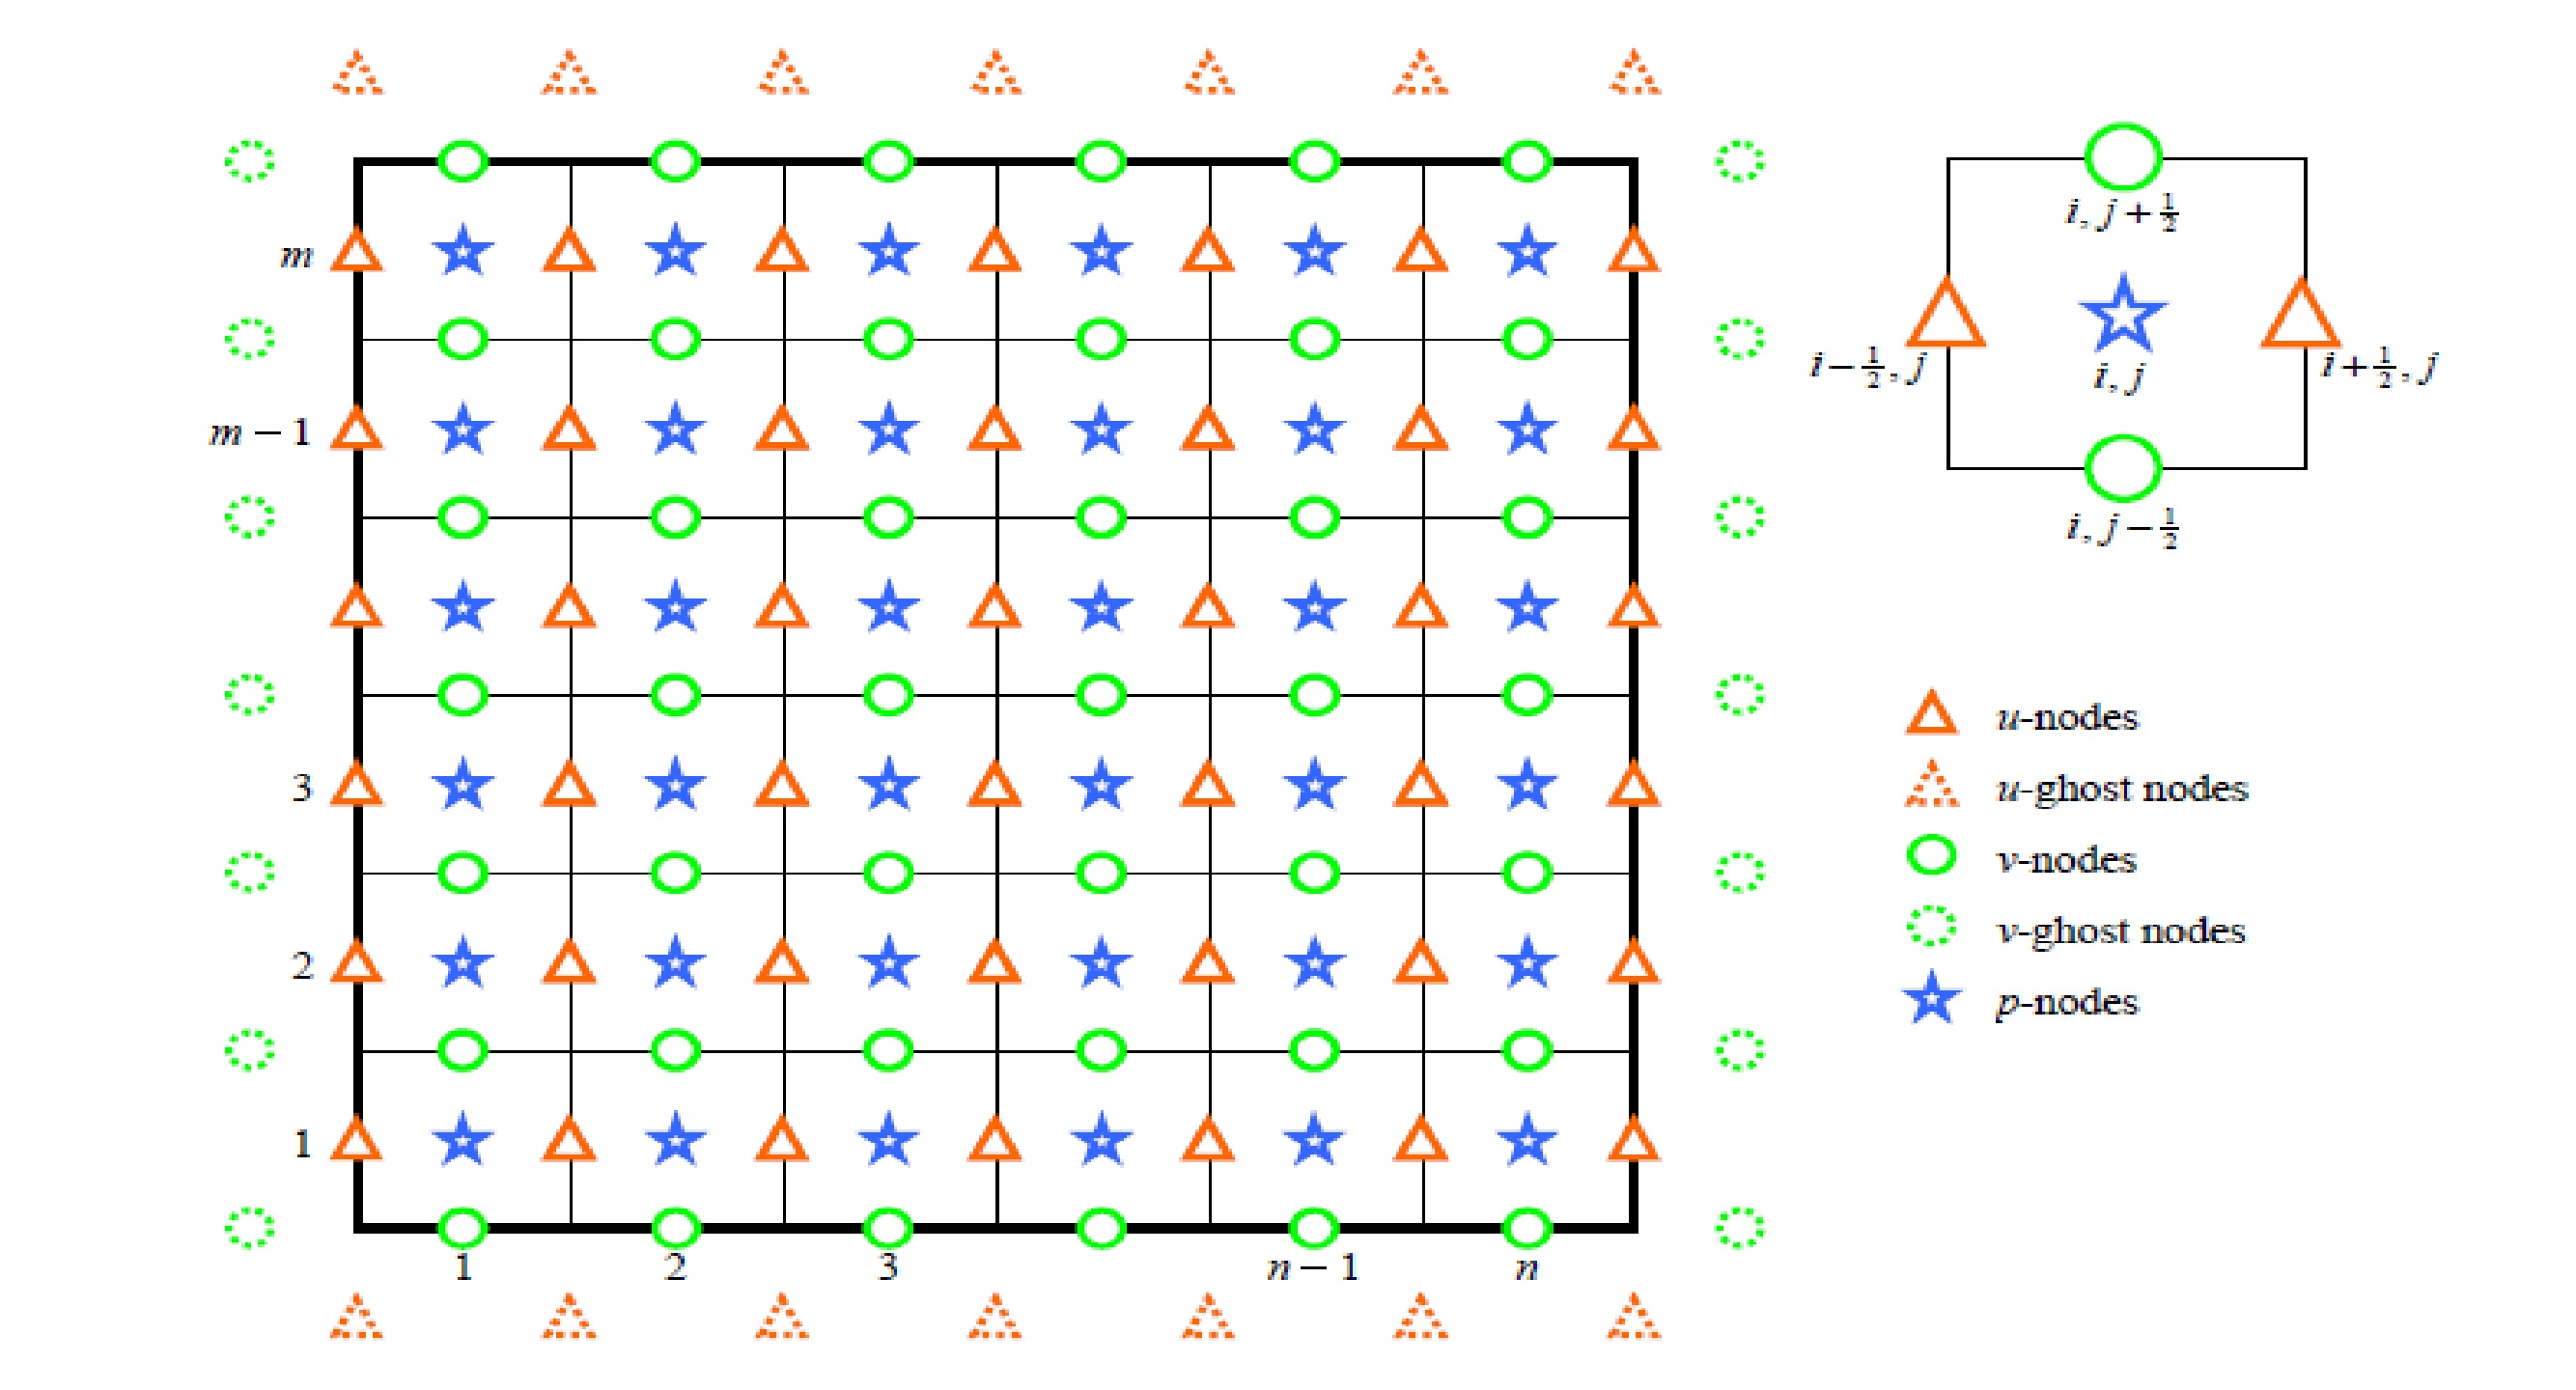
\includegraphics[width=6.5in]{C:/Users/HONGJI/Latex Home directory/staggered_grid.jpg}
	\caption{Picture of 2-D Staggered grid}\label{fig:6.1}
\end{figure}
The blue stars represent the pressure locations with the indexing of $i = 1,2,3,\cdots n$ and $j = 1,2,3,\cdots m$; the red triangles are the ``horizontal" $u$ velocities and they are assigned with half indices in the horizontal direction and integer indices in the vertical direction; the ``vertical" $v$ velocities on the other hand have integer indices in the vertical and half indices in the horizontal directions.
\begin{dgroup*}
\begin{dmath*}
u_{i-1/2,\,j} \condition{where $i = 1,2,3 \cdots n+1$ and $j = 1,2,3 \cdots m$}
\end{dmath*}
\begin{dmath*}
v_{i,\,j-1/2} \condition{where $i = 1,2,3 \cdots n$ and $j = 1,2,3 \cdots m+1$}
\end{dmath*}
\end{dgroup*}

The boundary points are those stored at the edge of the domain. For instance, the $u$ velocities have west and east boundary points with indices of West: ($i=\dfrac{1}{2},j$) and East: ($i=n+\dfrac{1}{2},j$); $v$ velocities have North and South boundaries points with indices ($i,j=\dfrac{1}{2}$) for South and ($i,j=m+\dfrac{1}{2}$) for North; pressure on the other hand only have interior points.\\
Below is a summary of spatial derivatives for a staggered grid
\begin{equation}
\begin{cases}
\dfrac{\partial u}{\partial x}|_{i-1/2,\,j} = \dfrac{u_{i+1/2,\,j} - u_{i-3/2,\,j}}{2\Delta x} + \mathcal{O}(\Delta x^2)\\
\dfrac{\partial v}{\partial y}|_{i,\,j-1/2} = \dfrac{v_{i,\,j+1/2} - v_{i,\,j-3/2}}{2\Delta y} + \mathcal{O}(\Delta y^2)\\
\textbf{u}(x,y,t=0) = \textbf{u}_0\,\,\,\text{   $x,\,y\,\in \Omega$}\\
\textbf{u}(x,y,t) = \textbf{u}_b\,\,\,\text{   $x,\,y\,\in \partial\Omega$ and $t\,\in [0,T]$}
\end{cases}
\end{equation} 
The derivatives can be calculated nicely in interior points however it is less straightforward to do so at the boundary points. For instance, if we want to know $\dfrac{\partial u}{\partial y}|_{i-1/2,1}$ next to the South boundary then this involves the up and down $u$ values with index $i-\dfrac{1}{2},0$ and $i=\dfrac{3}{2},2$. However $u_{i-1/2,0}$ simply does not exist because it is outside our domain. Can we ignore it? obviously not because it is needed to carry out the calculations. The inability to specify boundary values is one of the major drawbacks of staggered mesh grids. To tackle this problem, many people have used the concept of ``ghost cells" where we give $u$ a value at location ($-\dfrac{1}{2},j$). Then the derivative operations can be conducted as normal as the interior points. Therefore interpolation is needed to determine the ``ghost cell" values. Commonly, people have used 2 points average to calculate them. However this only gives first order accuracy and degrades the global spatial convergence error. To avoid this, higher order interpolations are needed. Robert has used a cubic polynomial interpolation to guarantee second order accuracy all the way up to the boundary \cite{sayenavierstokesmodule}. The formula can be derived by using Taylor expansion at the boundary point with the value of 3 interior points and the ghost cell. Then after rearrangement and cancelling of other function derivatives we derived a formula for ``ghost cells":\\
\begin{equation}
u_{i-1/2,0} = \dfrac{16}{5} u_{i-1/2,1/2} - 3 u_{i-1/2,1} + u_{i-1/2,2} - \dfrac{1}{5}u_{i-1/2,3}
\end{equation}\\
The velocity value at the corner e.g. $u_{i-1/2,1/2}$ are boundary points which will be given by the Dirichlet boundary condition for $u$. Its North counterpart is calculated similarly:\\
\begin{equation}
u_{i-1/2,m+1} = \dfrac{16}{5} u_{i-1/2,m+1/2} - 3 u_{i-1/2,m} + u_{i-1/2,m-1} - \dfrac{1}{5}u_{i-1/2,m-2}
\end{equation}\\
The ``ghost cells" of $v$ velocities are also derived using the same methodology:\\
\begin{equation}
v_{0,j-1/2} = \dfrac{16}{5} u_{1/2,j-1/2} - 3 u_{1,j-1/2} + u_{2,j-1/2} - \dfrac{1}{5}u_{3,j-1/2}
\end{equation}
\begin{equation}
v_{n+1,j-1/2} = \dfrac{16}{5} u_{n+1/2,j-1/2} - 3 u_{n,j-1/2} + u_{n-1,j-1/2} - \dfrac{1}{5}u_{n-2,j-1/2}
\end{equation}\\
Indeed, when writing programs (e.g Python) we cannot work with ``half indices". Therefore a special treatment of index is needed. For instance, we can double the index values ($i \Rightarrow 2i,\,j \Rightarrow 2j$) so that half indices are transformed to integers. In our case, for the sake of simplicity, a re-indexing was used. Looking at the staggered grid again, by joining the triangles together (including ghost cells) we extract a grid for $u$ velocities. Then Python indexing can be used here. For instance, West boundary points with staggered grid indices ($i=\dfrac{1}{2},j$) now have indices ($i=0,j$) in our new grid. Same strategy is used for $v$ and pressure too. It is worth to point out that the North and South are flipped over between the staggered grid and Python grid.

\subsection{Discretisation of Convective and Diffusive terms}
Because for centered differencing, we want to calculate all of our variables ($u,\,v$ and $p$) at half time indices. Therefore a temporal discretisation of convective and diffusive terms are also needed. In this section we will illustrate the temporal and spatial discretisation of the non-linear convection and diffusion terms which we have neglected in the previous chapters.\\
An explicit second order Adam Bashforth scheme is used to discretise the Convective term $\left[(\textbf{u}\cdot\nabla)\textbf{u}\right]^{k+1/2}$. Here $k$ is used for time iterations to distinguish with the spatial indices.
\begin{equation}
\left[(\textbf{u}\cdot\nabla)\textbf{u}\right]^{k+1/2} = \dfrac{3}{2}\left[(\textbf{u}\cdot\nabla)\textbf{u}\right]^k - \dfrac{1}{2}\left[(\textbf{u}\cdot\nabla)\textbf{u}\right]^{k-1}
\end{equation}
The spatial discretisation follows from our first subsection with a change of indices to fit with the staggered mesh grid.\\
For $u$ velocities which live on the triangles, their spatial discretisation is:
\begin{dgroup*}
\begin{dmath*}
\left[(\textbf{u}\cdot\nabla)\textbf{u}\right]_{i-1/2,j} = u_{i-1/2,j}\,\dfrac{u_{i+1/2,j} - u_{i-3/2,j}}{2\Delta x} + v_{i-1/2,j}\,\dfrac{u_{i-1/2,j+1} - u_{i-1/2,j-1}}{2\Delta y}
\end{dmath*}
\intertext{\\
However because in staggered grid, $v$ and $u$ are stored at different locations and hence spatial interpolation is again needed to compute $v_{i-1/2,j}$. This time a 4 point average will suffice for second order accuracy.\\
}
\begin{dmath*}
v_{i-1/2,j} = \dfrac{v_{i,j+1/2}+v_{i-1,j+1/2}+v_{i,j-1/2}+v_{i-1,j-1/2}}{4}
\end{dmath*}
\end{dgroup*}
Similarly for the $v$ component:
\begin{dgroup*}
\begin{dmath*}
\left[(\textbf{v}\cdot\nabla)\textbf{v}\right]_{i,j-1/2} = u_{i,j-1/2}\,\dfrac{v_{i+1,j-1/2} - v_{i-1,j-1/2}}{2\Delta x} + v_{i,j-1/2}\,\dfrac{v_{i,j+1/2} - v_{i,j-3/2}}{2\Delta y}
\end{dmath*}
\intertext{\\
Once again 4 point average is used to compute $u_{i,j-1/2}$ which we do not have direct access.
\\}
\begin{dmath*}
u_{i,j-1/2} = \dfrac{u_{i-1/2,j}+u_{i+1/2,j}+u_{i-1/2,j-1}+u_{i+1/2,j-1}}{4}
\end{dmath*}
\end{dgroup*}
There are other ways to treat the linear convective terms. For instance, we can put it into conservation form and use upwind scheme.\\
Now for the diffusive terms we have used the unconditionally stable Crank Nicholson method
\begin{equation}
\nabla^2 \textbf{u}^{k+1/2} = \nabla^2\,(\textbf{u}^*+\textbf{u}^k)
\end{equation}
where $\nabla^2 \textbf{u}$ is discretised as
\begin{dgroup*}
\begin{equation*}
\nabla^2 u = \dfrac{u_{i+1/2,j} - 2u_{i-1/2,j}+u_{i-3/2,j}}{\Delta x^2}+\dfrac{u_{i-1/2,j+1} - 2u_{i-1/2,j}+u_{i-1/2,j-1}}{\Delta y^2}
\end{equation*}
\begin{dmath*}
\nabla^2 v = \dfrac{v_{i+1,j-1/2} - 2v_{i,j-1/2}+v_{i-1,j-1/2}}{\Delta x^2}+\dfrac{v_{i,j+1/2} - 2v_{i,j-1/2}+_{i,j-3/2}}{\Delta y^2}
\end{dmath*}
\end{dgroup*}

the divergence of velocity is a scalar field and hence needs to match up with the locations of pressure points (the stars). it is calculated as:
\begin{equation*}
\nabla \cdot \textbf{u}_{i,j} = \dfrac{u_{i+1/2,j} - u_{i-1/2,j}}{\Delta x} + \dfrac{v_{i,j+1/2} - v_{i,j-1/2}}{\Delta y}
\end{equation*}

The gradient of pressure on the other hand is a vector field and hence needs to match up with the locations of velocities (triangles and circles). Hence it is calculated as follows:\\
x component:
\begin{dgroup*}
\begin{dmath*}
\partial_x p_{i-1/2,j} = \dfrac{p_{i,j} - p_{i-1,j}}{\Delta x}
\end{dmath*}
\begin{dmath*}
\partial_y p_{i,j-1/2} = \dfrac{p_{i,j} - p_{i,j-1}}{\Delta y}
\end{dmath*}
\end{dgroup*}

\subsection{Linear system solvers}
Now with every individual terms fully discretised and the introduction of intermediate velocity fields the momentum equation becomes:
\begin{equation}
\dfrac{\textbf{u}^* - \textbf{u}^n}{\Delta t} = -\nabla p^{n-1/2} -\dfrac{3}{2}\left[(\textbf{u}\cdot\nabla)\textbf{u}\right]^k + \dfrac{1}{2}\left[(\textbf{u}\cdot\nabla)\textbf{u}\right]^{k-1} + \dfrac{1}{2R}(\textbf{u}^*+\textbf{u}^n) + F^{n+1/2}
\end{equation}
where $F^{n+1/2}$ represents the external forcing, e.g. gravity.\\
Because we are working with Alg 2 method, hence we have taken the pressure approximation to be $q = p^{n-1/2}$.\\

Because of the implicit treat of diffusive terms, the intermediate velocity field must be solved as a linear system.\\
Further rearrange the momentum equation:
\begin{equation}
\left(I - \dfrac{\Delta t}{2R}\nabla^2\right)\textbf{u}^* = \textbf{u}^n + \Delta t\left(-\nabla p^{n-1/2} -\dfrac{3}{2}\left[(\textbf{u}\cdot\nabla)\textbf{u}\right]^k + \dfrac{1}{2}\left[(\textbf{u}\cdot\nabla)\textbf{u}\right]^{k-1} + \dfrac{1}{2R}(\textbf{u}^*+\textbf{u}^n) + F^{n+1/2} \right)
\end{equation}
Now with the Laplacian fully discretised, the problem above becomes a linear system:
\begin{equation}
A\textbf{u}^* = \textbf{b}
\end{equation}
where $A = \left(I - \dfrac{\Delta t}{2R}\nabla^2\right)$ and $\textbf{b}$ equals to the right hand side of the above equation. We use Algebraic multi-grid (AMG) method provided in Scipy to solve it.\\

As mentioned in previous chapters, the auxiliary field $\phi$ is solved as a Poisson equation which is a directly resulted from the projection:
\begin{dgroup}
\begin{dmath}
\nabla^2 \phi = \dfrac{1}{\Delta t}\nabla \cdot \textbf{u}^*
\end{dmath}
\intertext{with boundary condition}:
\begin{dmath}
\textbf{n} \cdot \nabla \phi = 0
\end{dmath}
\end{dgroup}
\textbf{Normalisation approach.}\\

This Poisson equation is also solved by algebraic multi-grid method. However care must be taken as the above equation with the Neumann boundary condition gives unique solution of $\phi$ only up to the addition of a constant. Hence we must find a way to recover the exact solution. We basically needs an extra constraint additional to the Poisson equation.\\

Although not discussed in the literature of Projection methods, we infer that a normalisation process is also implemented in the literature by researchers.\\

There are many choices of normalisation. One common ways is forcing the $\phi$ to satisfies an integral constraint:
\begin{equation}
\int_{\Omega}\,\int_{\Omega}\,\phi \,\,\, dx dy = 0
\end{equation}
However this approach involves calculating integrals and due to the limited timing we did not use it. This could be done in future researches.\\

Now regardless of what normalisation method we use, we should first note the relation between the exact $\phi$ and the numerical $\phi$ obtained from solving the Poisson equation.
\begin{equation}
\phi^{n+1}_{nu} = \phi^{n+1}_{ex} + a
\end{equation}
where the subscripts ``nu" and ``ex" stands for numerical and exact solutions respectively. Because of non-uniqueness there is no ``exact" $\phi$ solution, here exact refers to the one required by the projection method. Other $\phi$ solutions would causing the pressure to converge differently.\\

In practice during every time iteration, $\phi^{n+1}_{nu}$ is solved using the Poisson equation with the zero Neumann boundary condition. Because the Poisson equation with Neumann boundary condition does not guarantee uniqueness of $\phi$, hence we need to think what other constraints it must satisfy in the projection methods. In turns out that $\phi$ satisfies the pressure update equation! Rearrange \eqref{eg:general 2nd pressure update} and substitute into the above equation we obtained an expression for the constant $a$:
\begin{dmath}
a = \phi^{n+1}_{nu} - \dfrac{\Delta t}{2R} \nabla^2 \phi^{n+1} - (p^{n+1/2} - p^{n-1/2})
= \phi^{n+1}_{nu} - \dfrac{1}{2R} \nabla \cdot \textbf{u}^* - (p^{n+1/2} - p^{n-1/2})
\end{dmath}

This requires the knowledge of $p^{n+1/2}$ which of course we don't have when solving for $\phi^{n+1}$! However remember that $a$ is just a constant added to $\phi$ (and pressure), hence if we know the the pressure field at one point in domain then we can fully recover $a$. This point is arbitrary, but in practice, it is usually chosen along the boundary or center or any other points easily accessed. Therefore we need to impose a ``partial" Dirichlet condition on pressure. It is partial because we only require the knowledge of one point in space. In this section, we have chosen the point from the boundary $(x,y) \in \partial \Omega$.\\

\begin{dmath}\label{eq:normalisation constant for Alg 2}
a = \phi^{n+1}_{nu}|_{(x,y)\in \partial\Omega} - \dfrac{1}{2R} \nabla \cdot \textbf{u}^*|_{(x,y)\in \partial\Omega} - (p^{n+1/2} - p^{n-1/2})|_{(x,y)\in \partial\Omega}
\end{dmath}

Practically in order to ensure consistency we take 2 to 4 points along each boundary or corner and taking their average. \\

Let's consider a simple forced flow problem just for illustration purposes. The analytical solution of pressure ($p = \sin(t)\cos(\pi x)\sin(\pi y)$) indicates the North and South boundaries ($y=\pm 1$) are essentially zero for domain $[-1,1]^2$. Therefore naturally one can consider homogeneous Dirichlet boundary condition for pressure variable along these directions. Then by picking one arbitrary point along the boundary (for instance $y=1$ and $x$ is arbitrary) our equation for $a$ simplifies:
\begin{equation*}
a = \phi^{n+1}_{nu}\,(x,1) \,\,\,-\,\,\, \dfrac{1}{2R} \nabla \cdot \textbf{u}^*\,(x,1)
\end{equation*}
In the case of Staggered grids the spatial point $(x,1)$ refers to the coordinate: $(i,\,\dfrac{1}{2})$. Further dropping the time index for convenience we obtained:
\begin{equation*}
a = \phi^{nu}_{i,\,1/2} \,\,\,-\,\,\, \dfrac{1}{2R} \nabla \cdot \textbf{u}^*_{i,\,1/2}
\end{equation*}

However in Staggered grids, the coordinate ($i,\,1/2$) is along the top edge of the grid and no pressure is stored at this point (pressure is stored at ($i,\,j$) locations). Therefore interpolation from nearby cells are needed. This introduces spatial interpolation error and hence care must be taken to avoid accumulation of spatial errors.\\

In this case, we use a 3rd order cubic interpolation for $\phi^{nu}_{i,\,1/2}$ from 3 nearby points: $\phi^{nu}_{i,\,1}$, $\phi^{nu}_{i,\,2}$ and $\phi^{nu}_{i,\,3}$. Cubic interpolation is needed to ensure the first order derivative of $\phi^{nu}_{i,\,1/2}$ is also second order accurate along the boundary. By Taylor expanding $\phi^{nu}_{i,\,1}$, $\phi^{nu}_{i,\,2}$ and $\phi^{nu}_{i,\,3}$ at location ($i,\,1/2$) up to order $\mathcal{O}(\Delta t^3)$ we obtained an interpolation formula for $\phi^{nu}_{i,\,1/2}$ as

\begin{equation}
\phi^{nu}_{i,\,1/2} = \dfrac{15}{8}\phi^{nu}_{i,1} - \dfrac{5}{4}\phi^{nu}_{i,\,2}+\dfrac{3}{8}\phi^{nu}_{i,\,3}
\end{equation}
Exactly the formula can be used for $\nabla \cdot \textbf{u}^*$ since they are stored at the same locations as $\phi$.\\

Then the exact $\phi^{n+1}$ can be obtained by subtracting $a$ from $\phi^{n+1}_{nu}$ point-wisely. Thus we minus the same constant $a$ on every point of $\phi^{nu}$. Then the correct pressure can be recovered and we call it the ``Normalised Pressure". This in theory should fix the problem of error of error enlargement at finer grids. And this method indeed works as we shall see shortly!\\

For Projection method Alg 3, exactly the same process is used. In fact the expression for the normalisation constant $a$ is identical to that of Alg 2 \eqref{eq:normalisation constant for Alg 2} except the term $(p^{n+1/2} - p^{n-1/2})$ drops out since the pressure approximation $q$ is zero now.\\

For Gauge method, exactly the same procedure can be implemented too. From solving the Poisson equation \eqref{eq:Gauge pressure update} numerically we know that:
\begin{equation}
\chi^{n+1}_{nu} = \chi^{n+1}_{ex} + b\,\,\,\text{ and }\,\,\,\chi^{n}_{nu} = \chi^n_{ex} + c
\end{equation}
where $b$ and $c$ are constants. They are generally not equal and hence Gauge method also suffers from the non-uniqueness problem.\\

Again the point where we evaluate $b$ and $c$ is arbitrary, so let's use the same one considered above (note the analytical pressure is therefore still zero at this point).\\
Substitute the expression of $\chi_{nu}$ into the pressure update equation \eqref{eq:Gauge pressure update} and rearranging we obtained:
%\begin{equation}
%b - c = \chi^{n+1,\,\,\,nu}_{i,\,1/2} - \chi^{n,\,\,\,nu}_{i,\,1/2} + \dfrac{\Delta t}{2 R}(\nabla \cdot \textbf{m}^{n+1}_{i,\,1/2} + \nabla \cdot \textbf{m}^n_{i,\,1/2}) - p^{n+1/2}_{i,\,1/2}
%\end{equation}
\begin{equation}
b - c = \left(\chi^{n+1,\,\,\,nu} - \chi^{n,\,\,\,nu}\right)|_{(x,y)\in \partial\Omega} + \dfrac{\Delta t}{2 R}\left(\nabla \cdot \textbf{m}^{n+1} + \nabla \cdot \textbf{m}^n \right)|_{(x,y)\in \partial\Omega} - p^{n+1/2}|_{(x,y)\in \partial\Omega}
\end{equation}

\subsection{update velocity and pressure.}
This is the easiest step in the process. According to \eqref{eg:general 2nd velocity update} the velocities are updated as follows:\\
new $u$ velocity:
\begin{dgroup}
\begin{dmath}
u^{k+1}_{i-1/2,j} = u^*_{i-1/2,j} - \Delta t \dfrac{\partial p}{\partial x}|_{i-1/2,j} = u^*_{i-1/2,j} - \Delta t \,\dfrac{p_{i,j} - p_{i-1,j}}{\Delta x}
\end{dmath}
\intertext{and new $v$ velocity}
\begin{dmath}
v^{k+1}_{i,j-1/2} = u^*_{i,j-1/2} - \Delta t \dfrac{\partial p}{\partial y}|_{i,j-1/2} = u^*_{i,j-1/2} - \Delta t \,\dfrac{p_{i,j} - p_{i,j-1}}{\Delta y}
\end{dmath}
\end{dgroup}

and finally pressure:
\begin{equation}
p^{n+1/2}_{i,j} = p^{n-1/2}_{i,j} + \phi^{n+1}_{i,j} - \dfrac{\Delta t}{2R}\nabla^2\phi^{n+1}_{i,j} = p^{n-1/2}_{i,j} + \phi^{n+1}_{i,j} - \dfrac{1}{2R}\nabla \cdot \textbf{u}^*_{i,j}
\end{equation}